\documentclass{article}
\usepackage[margin=1in]{geometry}
\usepackage{amsmath,amssymb,amsthm,mathtools,bm}
\usepackage{tikz,pgfplots}
\pgfplotsset{compat=1.18}
\usepackage{hyperref}
\newtheorem{theorem}{Theorem}
\begin{document}
\section*{Math PDF toolchain check}
\begin{theorem}[Gaussian integral]
For $a>0$, $\int_{-\infty}^{\infty} e^{-ax^2}\,dx=\sqrt{\pi/a}$.
\end{theorem}
\begin{align}
\nabla\cdot\bm{E}&=\frac{\rho}{\varepsilon_0}, &
\mathbb{E}[X]&=\sum_{k=0}^{\infty}k\,\mathbb{P}(X=k),\\
A&=\begin{pmatrix}1&2\\0&1\end{pmatrix}, &
f(x)&=\begin{cases}x^2&x\geq0,\\-x&x<0.\end{cases}
\end{align}
\begin{center}
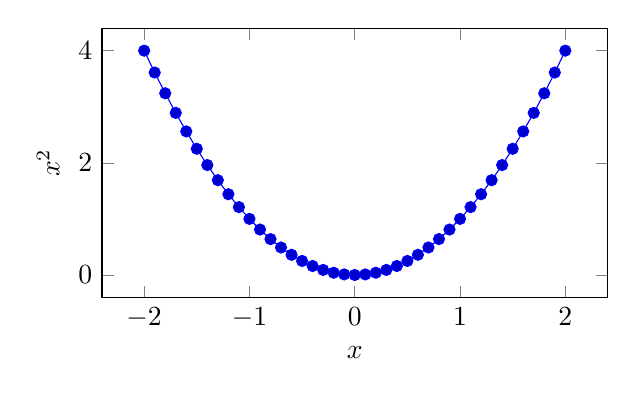
\begin{tikzpicture}
\begin{axis}[width=8cm,height=5cm,xlabel={$x$},ylabel={$x^2$},domain=-2:2,samples=41]
\addplot {x^2};
\end{axis}
\end{tikzpicture}
\end{center}
A reference to the standard text~\cite{knuth}.
\bibliographystyle{plain}
\bibliography{latex-smoke}
\end{document}
